\documentclass[a4paper,12pt]{article}
\usepackage{polski}
\usepackage[utf8]{inputenc}
\usepackage[left = 3cm, right = 3cm, top = 2cm, bottom = 2cm]{geometry}
\usepackage{enumerate}
\usepackage{amssymb}		% pakiet do symboli
\usepackage{mathtools}		% pakiet do matmy (rozszerza amsmath)
\usepackage{enumitem}		% punktowanie (a), (b), ...
\usepackage{nopageno}		% brak numerow stron
\usepackage{graphicx}		% wstawianie obrazkow
\usepackage{float}			% wstawianie obrazkow w dowolnym miejscu
\usepackage{caption}
\usepackage{subcaption}
\usepackage{titling}
\usepackage{algpseudocode}	
\usepackage{algorithm}

% nowe komendy dla wygodniejszego pisania :)

\newcommand{\floor}[1]{\left\lfloor #1 \right\rfloor}	% podłoga
\newcommand{\ceil}[1]{\left\lceil #1 \right\rceil}		% sufit
\newcommand{\fractional}[1]{\left\{ #1 \right\}}		% część ułamkowa {x}
\newcommand{\abs}[1]{\left| #1 \right|}					% wartosc bezwzgledna / moc
\newcommand{\set}[1]{\left \{ #1 \right \}}				% zbiór elementów {a,b,c}
\newcommand{\pair}[1]{\left( #1 \right)}				% para elementów (a,b)
\newcommand{\Mod}[1]{\ \mathrm{mod\ #1}}				% lekko zmodyfikowane modulo
\newcommand{\comp}[1]{\overline{ #1 }} 					% dopełnienie zbioru 
\newcommand{\annihilator}{\mathbf{E}}					% operator E
\newcommand{\seqAnnihilator}[1]{\annihilator \left\langle #1 \right\rangle} % E(a_n)
\newcommand{\sequence}[1]{\left\langle #1 \right\rangle} % <a_n>
\DeclareMathOperator{\lcm}{lcm}							% obsługa lcm w mathmode

\begin{document}
\noindent \textbf{Matematyka dyskretna L, Lista 7 - Tomasz Woszczyński}\newline

\noindent \newline \textbf{Zadanie 1} \newline
Należy udowodnić, że liczba podziałów $(n+2)$-kąta wypukłego na płaszczyźnie na rozłączne trójkąty za pomocą $n-1$ nieprzecinających się przekątnych jest równa $n$-tej liczbie Catalana. \\

\noindent Wyobraźmy sobie podział najprostszych figur: weźmy trójkąt, nie możemy go podzielić w żaden sposób, gdyż nie istnieją w nim przekątne, stąd mamy tylko jedną możliwość. Dla kwadratu możemy poprowadzić tylko dwie przekątne, więc istnieją dwie możliwości podziału. \\

\noindent Weźmy teraz $n+2$-kąt wypukły i wybierzmy jeden z jego boków, następnie poprowadźmy z jego końców odcinki (przekątne) do jednego wierzchołka. Dzięki temu otrzymamy figury $F_1, F_2$ oraz trójkąt $T_1$, tak jak przedstawia poniższy rysunek.

\begin{figure}[H]
	\centering
	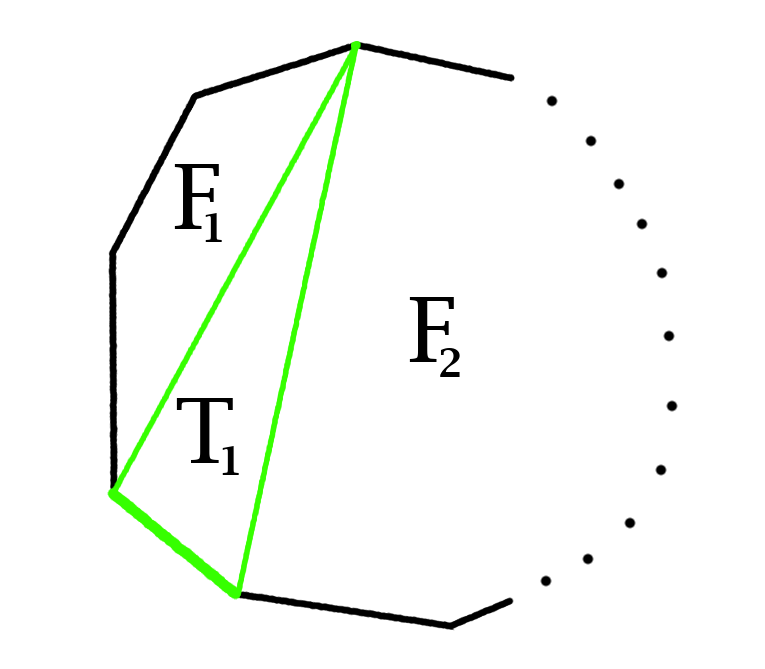
\includegraphics[width=0.5\textwidth]{Rysunki/l7z1.png}
\end{figure}

\noindent Figury $F_1$ oraz $F_2$ dzielimy dalej przekątnymi na rozłączne trójkąty, dopóki jest to możliwe. Jeśli rozpoczniemy podział od jednej ze stron wielokąta, będziemy uzyskiwali trójkąt oraz $i-1$ kąt, aż do ukończenia podziału całej figury. Oznaczmy te podziały przez $q_i$, wtedy liczbę możliwości podziału $n+2$-kąta wyraża wzór:
\[ q_{n+2} = q_{n+1} \cdot q_2 + q_{n} \cdot q_3 + q_{n-1} \cdot q_4 + \ldots + q_3 \cdot q_{n} + q_2 \cdot q_{n+1} \]

\noindent Można zauważyć, że po przeindeksowaniu $q_{n+2}$ o $2$ uzyskamy $C_n$, będący liczbą Catalana. Prościej mówiąc, szukana zależność to $q_{n+2} = C_n$, co należało udowodnić.


\newpage
\noindent \textbf{Zadanie 2} \newline
Określ liczbę drzew binarnych zawierających $n$ wierzchołków wewnętrznych. Wierzchołek drzewa binarnego ma zero lub dwóch synów. \\

\noindent Doprecyzujmy definicję węzła wewnętrznego - jest to węzeł, który posiada synów, a więc nie jest liściem. Na poniższym rysunku są to wierzchołki $V = \{ 1, 2, 3, 4, 5 \}$.

\begin{figure}[H]
	\centering
	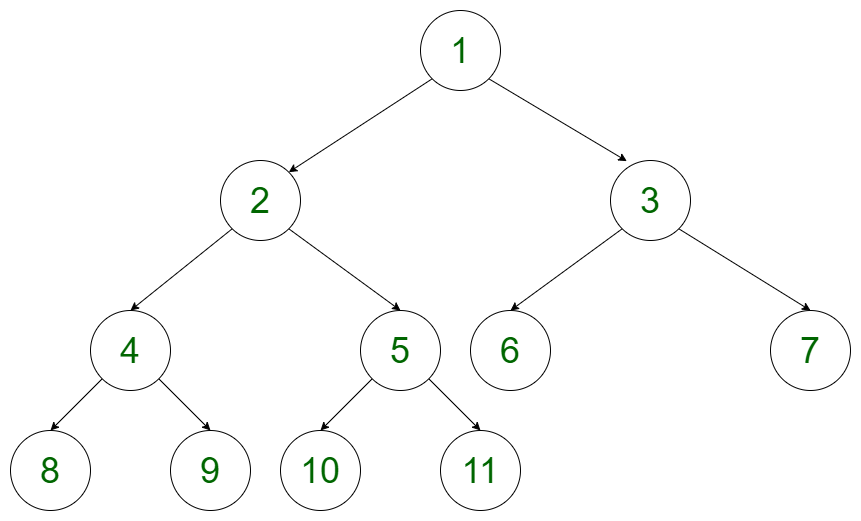
\includegraphics[width=0.75\textwidth]{Rysunki/l7z2.png}
\end{figure}

\noindent Przez $x_n$ oznaczmy liczbę drzew binarnych o $n$ wierzchołkach wewnętrznych.  Pojedynczy wierzchołek jest jedynym pełnym drzewem binarnym bez węzłów wewnętrznych, a więc $x_0 = 1$. Mając drzewo $T$ z co najmniej jednym wierzchołkiem wewnętrznym, możemy je jednoznacznie rozłożyć na dwa poddrzewa: lewe $T_L$ oraz prawe $T_R$. Oznaczmy przez $T_n$ rodzinę wszystkich drzew binarnych z $n$ węzłami wewnętrznymi oraz przez $T_{l, r}$ rodzinę wszystkich drzew, których podrzewa $T_L$ oraz $T_R$ mają odpowiednio $l$ oraz $r$ węzłów wewnętrznych. Wtedy mamy:
\[ \abs{T_{l, r}} = \abs{T_l \times T_r} = \abs{T_l} \cdot \abs{T_r} = x_l \cdot x_r \]

\noindent Zauważmy, że w lewym poddrzewie możemy mieć $0$ wierzchołków wewnętrznych, a w prawym $n-1$ (po rozdzieleniu względem wierzchołka wewnętrznego) lub $1$ w lewym i $n-2$ w prawym, itd. Sytuację taką możemy opisać jako sumę odpowiednich rodzin (zbiorów):
\[ T_n = T_{0, n - 1} \cup T_{1, n - 2} \cup T_{2, n - 3} \cup \ldots \cup T_{n-1, 0} \]
a po wcześniejszym przekształceniu ($\abs{T_{l, r}} = x_l \cdot x_r$), jako następującą sumę:
\[ x_n = x_0 \cdot x_{n-1} + x_1 \cdot x_{n-2} + \ldots + x_{n-1} \cdot x_0 = C_n \]
Oznacza to, że istnieje $C_n$ drzew binarnych o $n$ wierzchołkach wewnętrznych.

\newpage
\noindent \textbf{Zadanie 3} \newline
Ile niekrzyżujących się uścisków dłoni może wykonać jednocześnie $n$ par osób siedzących za okrągłym stołem? \\

\noindent Mamy $2n$ osób wykonujących jednocześnie $n$ nieprzecinających się uścisków dłoni. Ponumerujmy te osoby od $1$ do $2n$, aby precyzyjniej mówić o możliwych uściskach. Załóżmy więc, że osoba $1$ wybiera osobę $i$, wtedy pozostałe osoby $2, \ldots, i - 1$ oraz $i + 1, \ldots, 2n$ \textbf{muszą} tworzyć konfigurację, w której  również będą mogły uścisnąć dłonie bez przecięć, a więc żadna osoba nie będzie odizolowana od reszty. Łatwo wywnioskować, że $i$ musi być parzyste, weźmy więc $i = 2k$. \\

\noindent Wnioskowanie to przypomina problem nawiasowania. Ściślej, mamy do czynienia z $2n$ osobami (nawiasami) oraz $n$ uściskami (dobre pary nawiasów). Aby łatwiej mówić o uściskach, weźmy osoby $i, j$, a następnie podzielmy je sobie na uściski "wychodzące" dla $i < j$ oraz uściski "przychodzące" w przeciwnym przypadku. Uściski wychodzące oznaczać będziemy lewym nawiasem, a przychodzące - prawym. \\

\noindent Numerując wtedy osoby na okręgu od $1$, która pierwsza wyciąga rękę (uścisk wychodzący), nasz ciąg będzie zaczynał się lewym nawiasem, w przeciwnym wypadku mielibyśmy ciąg nawiasów rozpoczynający się od prawego nawiasu, co nie byłoby poprawne. Przykładowe odzworowanie przedstawiają poniższe rysunki.

\begin{figure}[H] % trzy rysunki przecinających się okręgów, wyśrodkowane w pionie
	\centering
	$\vcenter{\hbox{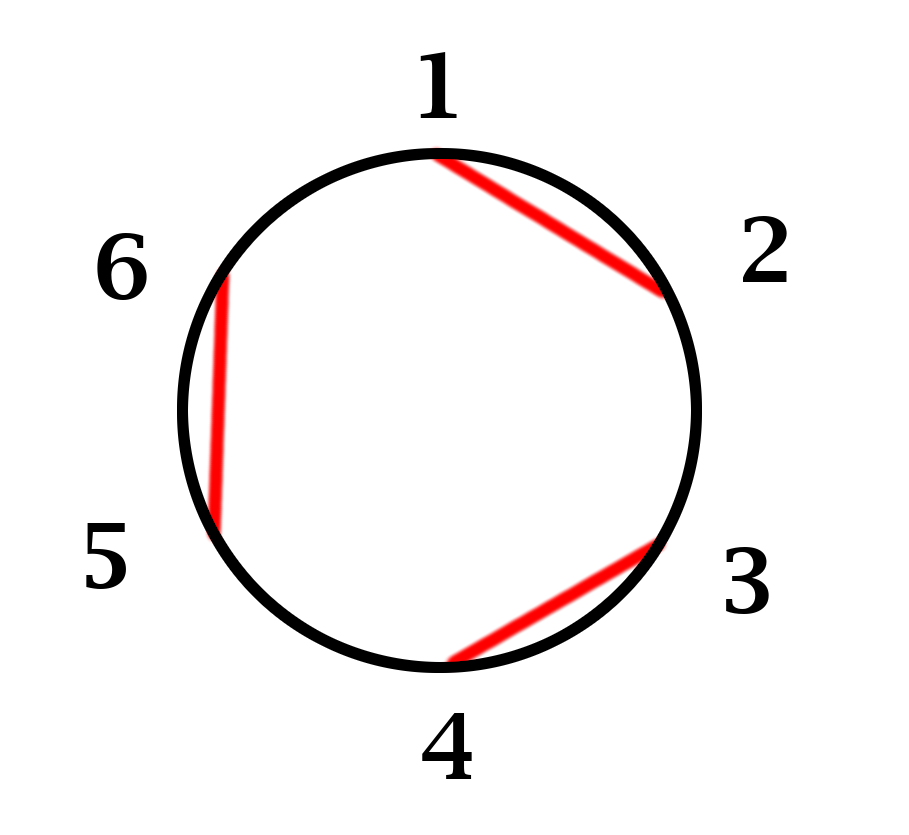
\includegraphics[width=.32\textwidth]{Rysunki/l7z3a.png}}}$
	$\vcenter{\hbox{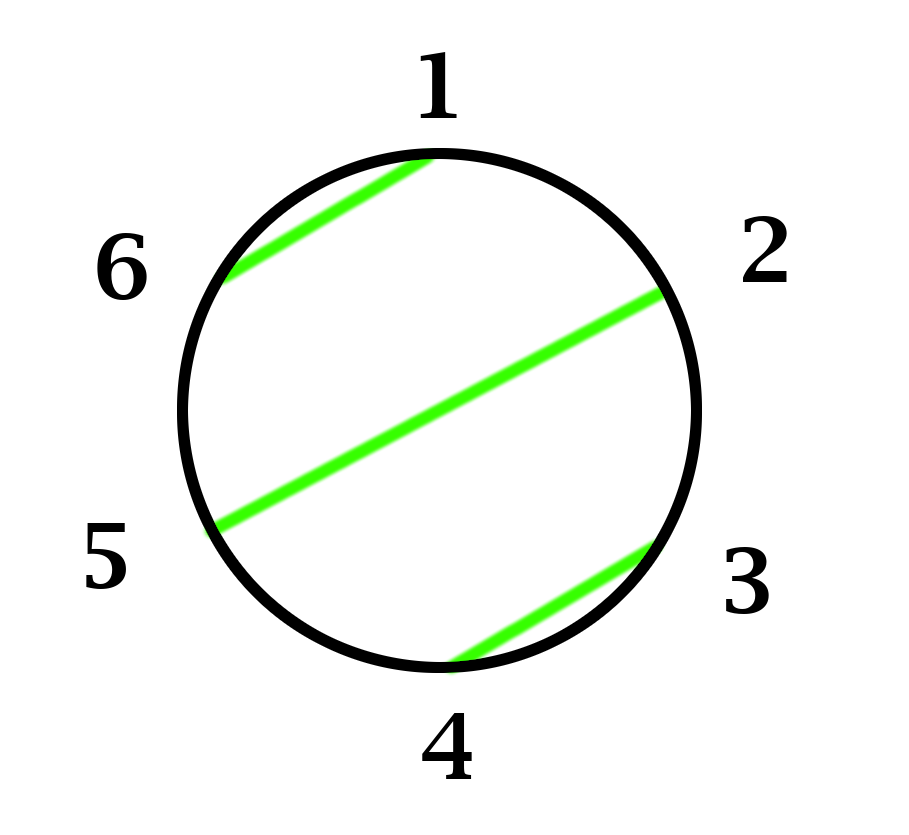
\includegraphics[width=.32\textwidth]{Rysunki/l7z3b.png}}}$
	$\vcenter{\hbox{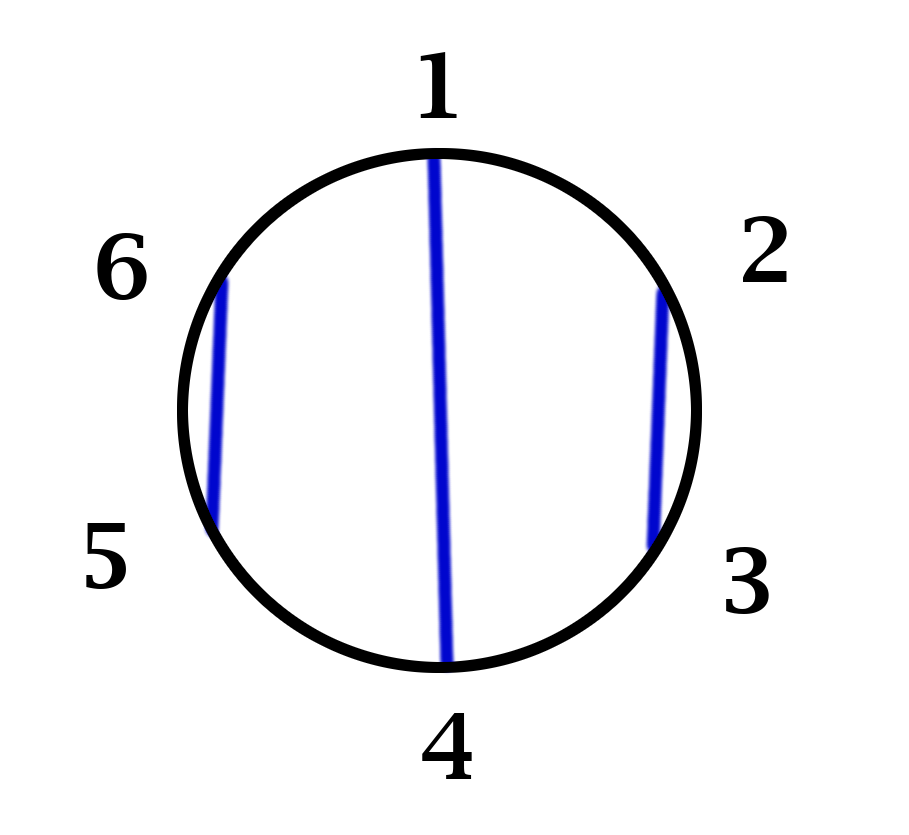
\includegraphics[width=.32\textwidth]{Rysunki/l7z3c.png}}}$
\end{figure}

\noindent Nawiasowaniem dla ustawienia czerwonego będzie $()()()$, dla zielonego $((()))$, a dla niebieskiego $(())()$. Można dostrzec, że im bardziej są od siebie oddalone (w sensie indeksów) osoby, tym więcej nawiasów odzwierciedlających uściski znajdzie się pomiędzy nimi.\\

\noindent Opisane wyżej odzworowanie jest bijekcją, dzięki czemu niekrzyżujących się uścisków dłoni dla $2n$ osób jest tyle samo, co dobrych nawiasowań dla $2n$ nawiasów. Jest to $n$-ta liczba Catalana wyrażona wzorem:
\[ C_n = \sum\limits_{i = 1}^{n} c_{i - 1} \cdot c_{n - i} \] 

\newpage
\noindent \textbf{Zadanie 5} \newline
Podaj funkcję tworzącą dla ciągu $\sequence{0, 0, 0, 1, 3, 7, 15, 31, \ldots}$.\\

\noindent Łatwo zauważyć, że zadany ciąg $\sequence{a_n}$ jest połączeniem dwóch ciągów $\sequence{b_n}$ i $\sequence{c_n}$:
\begin{align*}
    \sequence{b_n}  &= \sequence{0, 0, 1, 2, 4, 8, 16, 32, \ldots} \\
    \sequence{c_n}  &= \sequence{0, 0, -1, -1, -1, -1, -1, \ldots} \\
\end{align*} \\[-50pt]

\noindent Naszym zadaniem jest więc znalezienie funkcji tworzących $B(x)$ oraz $C(x)$ dla powyższych ciągów, a następnie dodanie ich do siebie, aby stworzyć funkcję $A(x)$. \\

\noindent Zacznijmy więc od ciągu $\sequence{b_n}$. Są to kolejne potęgi dwójki przesunięte o dwa miejsca w prawo. Ciąg $\sequence{2^n}$ wyraża $\frac{1}{1-2x}$, należy go jeszcze przesunąć o dwa miejsca w prawo, a więc całe wyrażenie pomnożyć przez $x^2$ (dla przesunięcia o $k$ miejsc jest to $x^k$, dowód w kolejnym zadaniu). Mamy więc:
\[ B(x) = x^2 \cdot \frac{1}{1 - 2x} = \frac{x^2}{1 - 2x} \]
 
\noindent Ciąg $\sequence{c_n}$ jest łatwiejszy do uzyskania. Weźmy funkcję tworzącą ciągu $\sequence{1, 1, 1, \ldots}$, pomnóżmy ją przez $-1$, aby uzyskać ciąg $\sequence{-1, -1, -1, \ldots}$, a następnie pomnóżmy przez $x^2$, aby przesunąć go o dwa miejsca w prawo, aby ostatecznie otrzymać $\sequence{0, 0, -1, -1, -1, \ldots}$. Otrzymujemy więc:
\[ C(x) = (-1) \cdot x^2 \cdot \frac{1}{1 - x} = \frac{-x^2}{1 - x} \]

\noindent Skorzystajmy teraz z zasady dodawania funkcji tworzących dla ciągów $\sequence{b_n}$ i $\sequence{c_n}$, dzięki czemu otrzymamy funkcję tworzącą ciągu $\sequence{a_n}$:
\[ A(x) = B(x) + C(x) = \frac{x^2}{1 - 2x} + \frac{-x^2}{1 - x} = \frac{x^3}{2x^2 - 3x + 1} \]

\newpage
\noindent \textbf{Zadanie 6} \newline
\textbf{Pytanie 1:} Niech $A(x)$ będzie funkcją tworzącą ciągu $\sequence{a_n}$. Pokaż, że funkcja tworząca ciągu $\sequence{b_n}$ postaci $\sequence{\underbrace{0, 0, \ldots, 0}_{k}, a_0, a_1, a_2, \ldots}$ jest $x^k \cdot A(x)$. \\

\noindent Wiemy, że funkcją tworzącą ciągu $\sequence{a_n}$ jest 
\[ A(x) = \sum\limits_{n=0}^{\infty} a_n x_n = a_0 x^0 + a_1 x^1 + a_2 x^2 + a_3 x^3 + \ldots \]
Załóżmy, że aby uzyskać funkcję tworzącą ciągu $\sequence{b_n}$, a więc ciągu $\sequence{a_n}$ przesuniętego o $k$ miejsc w prawo, należy pomnożyć $A(x)$ przez $x^k$. Udowodnię to indukcyjnie:
\begin{enumerate}
	\item Podstawa indukcyjna: $k = 0$ (brak przesunięcia), mamy wtedy
    \[ x^0 \cdot A(x) = 1 \cdot A(x) = B(x), \text{ więc się zgadza } \checkmark \]
	\item Krok indukcyjny: załóżmy, że dla $k$ zachodzi $B_k(x) = x^k \cdot A(x)$, pokażę, że dla $k+1$ zachodzi $B_{k+1}(x) = x^{k+1} \cdot A(x)$.
	\begin{align*}
        x^{k+1} \cdot A(x)  &= x \cdot x^k \cdot A(x) = x \cdot B_k(x) = \\
                            &= x \cdot \underbrace{\left(a_0 x^k + a_1 x^{k+1} + a_2 x^{k+2} + a_3 x^{k+3} + \ldots\right)}_{\text{ciąg przesunięty o } k} = \\
                            &= \underbrace{\left(a_0 x^{k+1} + a_1 x^{k+2} + a_2 x^{k+3} + a_3 x^{k+4} + \ldots\right)}_{\text{ciąg przesunięty o } k + 1} = \\
                            &= \sequence{\underbrace{0, 0, \ldots, 0}_{k + 1}, a_0, a_1, a_2, \ldots} = B_{k+1}(x)
    \end{align*}
\end{enumerate}
Udowodniliśmy, że przesunięcie ciągu o $k$ miejsc w prawo wyraża się jako $x^k \cdot A(x)$. \\

\noindent\textbf{Pytanie 2:} W jaki sposób otrzymać funkcję tworzącą ciągu $\sequence{c_n}$ postaci $\sequence{a_k, a_{k+1}, \ldots}$, czyli takiego, że $c_i = a_{k + i}$? \\

\noindent Mamy funkcję tworzącą ciągu $A(x)$, aby otrzymać ciąg przesunięty o $1$ w lewo (więc bez pierwszego wyrazu), należy odjąć pierwszy wyraz od $A(x)$, a następnie całość podzielić przez $x$. Dla $k$ wyrazów można to uogólnić do postaci:
\[ C(x) = \frac{A(x) - \left(a_0 x^0 + a_1 x^1 + \ldots + a_{k-1} x^{k-1}\right)}{x^k} = \sum\limits_{n=0}^{\infty} a_{n + k} x^n \]

\noindent Można to udowodnić indukcyjnie w sposób analogiczny do przesunięcia w prawo, jednak można przekształcić to wyrażenie algebraicznie, aby dojść do tego samego wniosku. Rozpiszmy więc kolejne kroki przesunięcia o $k$ w lewo:
\begin{align*}
    C(x)    &= \frac{A(x) - \left(a_0 x^0 + a_1 x^1 + \ldots + a_{k-1} x^{k-1}\right)}{x^k} = \\
            &= \frac{\left(a_0 x^0 + \ldots + a_{k-1} x^{k-1} + a_k x^k + \ldots\right) - \left(a_0 x^0 + a_1 x^1 + \ldots + a_{k-1} x^{k-1}\right)}{x^k} = \\
            &= \frac{a_k x^k + a_{k+1} x^{k+1} + a_{k+2} x^{k+2} + \ldots}{x_k} = \frac{x_k \cdot \left( a_k + a_{k+1} x^1 + a_{k+2} x^2 + \ldots \right)}{x_k} =  \\ 
            &= a_k x^0 + a_{k+1} x^1 + a_{k+2} x^2 + \ldots = \sum\limits_{n=0}^{\infty} a_{n + k} x^n, \text{ co kończy dowód.}
\end{align*}

\newpage
\noindent \textbf{Zadanie 7} \newline
Podaj postać funkcji tworzącej dla liczby podziałów liczby naturalnej $n$ (czyli rozkładów liczby $n$ na sumę składników naturlanych, gdy rozkładów różniących się kolejnością nie uważamy za różne):
\begin{enumerate}
    \item na dowolne składniki,
    \item na różne składniki nieparzyste,
    \item na składniki mniejsze od $m$,
    \item na różne potęgi liczby $2$.
\end{enumerate}

\noindent \textbf{Przykład 1:} Liczba rozkładów $n$ za pomocą dowolnej liczby składników naturalnych wyraża się funkcją tworzącą podaną na wykładzie, a więc jest to: 
\[ r_n = \prod\limits_{i = 1}^{\infty} \frac{1}{1 - x^i} \]

\noindent \textbf{Przykład 2:} Liczba rozkładów $n$ na różne składniki wyraża się wzorem
\[ rr_n = \prod\limits_{i = 1}^{\infty} (1 + x^i) \]
Nas jednak interesuje liczba rozkładów na różne składniki nieparzyste, dlatego musimy zmodyfikować potęgę przy $x$, aby w iloczynie występowały tylko nieparzyste:
\[ \prod\limits_{i = 1}^{\infty} (1 + x^{2i - 1}) \]

\noindent \textbf{Przykład 3:} Teraz chcemy otrzymać rozkład $n$ na składniki mniejsze od $m$. Modyifkujemy więc górną granicę iloczynu i korzystamy ze wzoru na $r_n$:
\[ \prod\limits_{i = 1}^{m - 1} \frac{1}{1 - x^i} \]

\noindent \textbf{Przykład 4:} Chcemy podzielić $n$ na składniki będące różnymi potęgami $2$. Wynik będzie korzystał z $rr_n$, jednak zmodyfikujemy znów potęgę stojącą przy $x$ w taki sposób, aby mieć kolejne potęgi $2$. Ostateczny wzór to:
\[ \prod\limits_{i = 1}^{\infty} (1 + x^{2^{i}}) \]

\end{document}